%% ─────────────────────────────────────────────────────────────────────────────
%% Anexo II — Evaluación de calibración: gráficas por piloto
%% ─────────────────────────────────────────────────────────────────────────────

\chapter{Evaluación de calibración: gráficas por piloto}
\label{ann:eval_calibracion}

Este anexo complementa la sección~\ref{sec:eval_calibracion} con la lectura individual de cada piloto sobre las carreras evaluadas de 2025. Primero se ofrecen los cuatro comentarios cualitativos por piloto; a continuación, la rejilla común con las series temporales del error firmado (figura~\ref{fig:eval_error_signed_all}); y, finalmente, un \textit{dumbbell} a página completa por piloto, en orden Norris, Piastri, Verstappen y Leclerc, con el tiempo total predicho (círculo blanco) y el tiempo real (círculo relleno) carrera a carrera, unidos por una línea fina del color del piloto y con el error firmado anotado a la derecha. La lectura agregada (MAPE, sesgo, distribución del error absoluto) se reserva al capítulo~\ref{cap:resultados}; aquí el foco es el comportamiento del motor en cada Gran Premio concreto.

% ──────────────── Comentarios por piloto ────────────────
\section*{Norris}
\label{ann:eval_NOR}

Norris cierra la temporada con un MAPE del 14{,}45\,\% y un sesgo medio de +682\,s sobre 24 carreras. El \textit{dumbbell} a página completa (figura~\ref{fig:eval_NOR_dumbbell}) permite localizar las dos divergencias mayores (Melbourne y Spa), donde el motor predice un tiempo cercano al nominal mientras que la carrera real se acorta por bandera roja o lluvia. La serie temporal del error firmado en el orden del calendario aparece en el primer panel de la figura~\ref{fig:eval_error_signed_all}.

\section*{Piastri}
\label{ann:eval_PIA}

Piastri es el piloto con mayor MAPE de los cuatro (14{,}57\,\%) y un sesgo medio de +688\,s sobre 23 carreras válidas. Su patrón temporal (segundo panel de la figura~\ref{fig:eval_error_signed_all}) es prácticamente paralelo al de su compañero de equipo Norris, lo que sugiere que el sesgo procede del motor y no de un perfil paramétrico del piloto. El \textit{dumbbell} correspondiente es la figura~\ref{fig:eval_PIA_dumbbell}.

\section*{Verstappen}
\label{ann:eval_VER}

Verstappen presenta un MAPE del 14{,}56\,\% y un sesgo medio de +692\,s sobre 23 carreras. El \textit{dumbbell} (figura~\ref{fig:eval_VER_dumbbell}) confirma que la sobreestimación se reparte de manera homogénea por el calendario, sin un circuito concreto que aporte un peso desproporcionado al sesgo global más allá de los casos extremos comunes a los cuatro pilotos. La serie temporal aparece en el tercer panel de la figura~\ref{fig:eval_error_signed_all}.

\section*{Leclerc}
\label{ann:eval_LEC}

Leclerc es el piloto mejor calibrado de los cuatro, con un MAPE del 13{,}53\,\% y un sesgo medio de +637\,s sobre 24 carreras. La mediana del error firmado se sitúa en +476\,s, la más baja del grupo, lo que se traduce en una franja de error más estrecha en el cuarto panel de la figura~\ref{fig:eval_error_signed_all}. El \textit{dumbbell} correspondiente es la figura~\ref{fig:eval_LEC_dumbbell}.

% ──────────────── Rejilla común: error firmado ────────────────
\clearpage
\begin{figure}[H]
\centering
\begin{subfigure}[t]{\textwidth}
  \centering
  \IfFileExists{Chapter5/images/error_signed_NOR.pdf}{%
    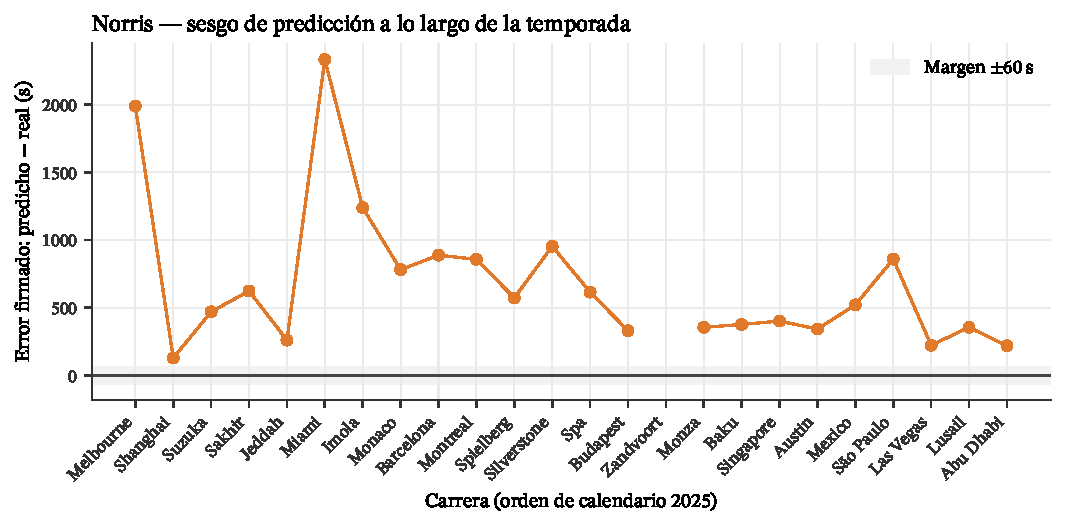
\includegraphics[width=0.9\linewidth,height=0.185\textheight,keepaspectratio]{Chapter5/images/error_signed_NOR.pdf}%
  }{\rule{0pt}{3cm}}
\end{subfigure}

\vspace{0.4em}

\begin{subfigure}[t]{\textwidth}
  \centering
  \IfFileExists{Chapter5/images/error_signed_PIA.pdf}{%
    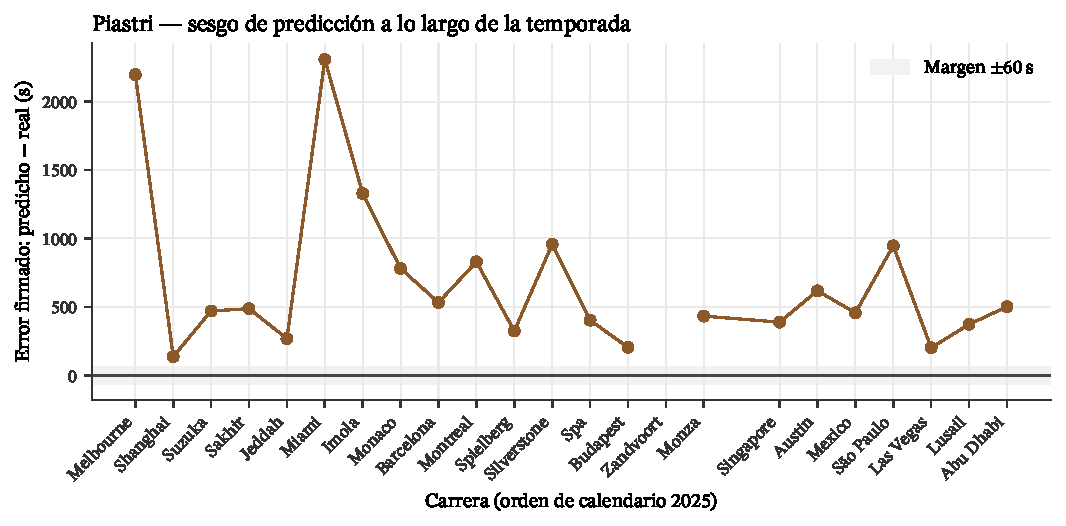
\includegraphics[width=0.9\linewidth,height=0.185\textheight,keepaspectratio]{Chapter5/images/error_signed_PIA.pdf}%
  }{\rule{0pt}{3cm}}
\end{subfigure}

\vspace{0.4em}

\begin{subfigure}[t]{\textwidth}
  \centering
  \IfFileExists{Chapter5/images/error_signed_VER.pdf}{%
    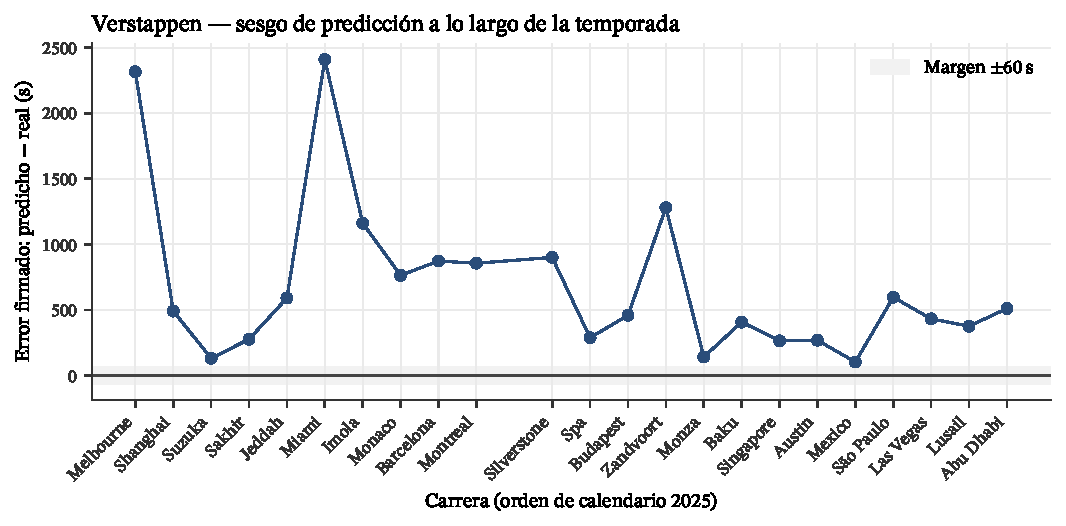
\includegraphics[width=0.9\linewidth,height=0.185\textheight,keepaspectratio]{Chapter5/images/error_signed_VER.pdf}%
  }{\rule{0pt}{3cm}}
\end{subfigure}

\vspace{0.4em}

\begin{subfigure}[t]{\textwidth}
  \centering
  \IfFileExists{Chapter5/images/error_signed_LEC.pdf}{%
    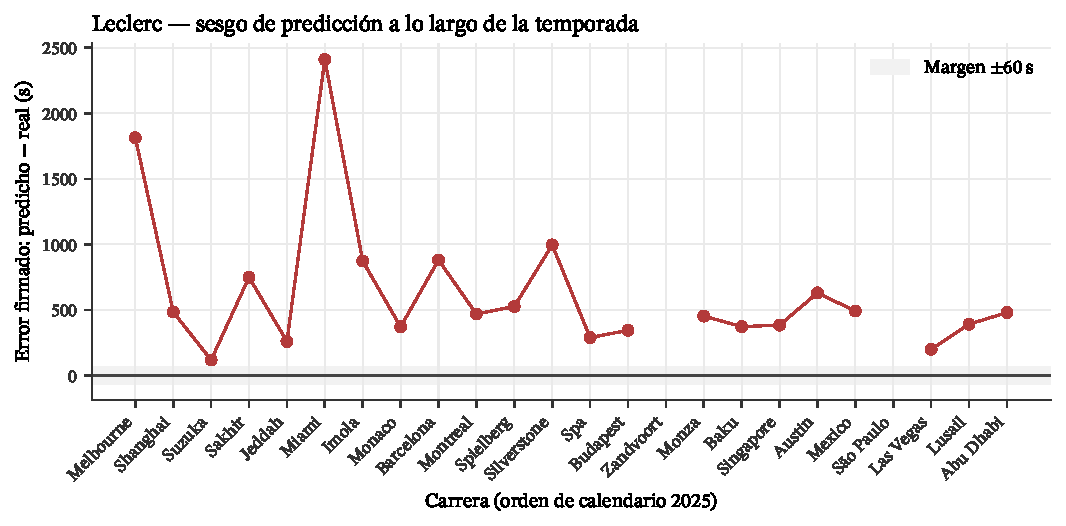
\includegraphics[width=0.9\linewidth,height=0.185\textheight,keepaspectratio]{Chapter5/images/error_signed_LEC.pdf}%
  }{\rule{0pt}{3cm}}
\end{subfigure}
\caption{Series temporales del error firmado predicho\,$-$\,real por piloto sobre las carreras evaluadas de 2025. En cada panel la franja gris marca el margen $\pm$\SI{60}{\second} aplicado por el motor frente a un evento de \textit{safety car}.}
\label{fig:eval_error_signed_all}
\end{figure}

% ──────────────── Dumbbells a página completa ────────────────
\clearpage
\begin{figure}[H]
\centering
\IfFileExists{Chapter5/images/dumbbell_NOR.pdf}{%
  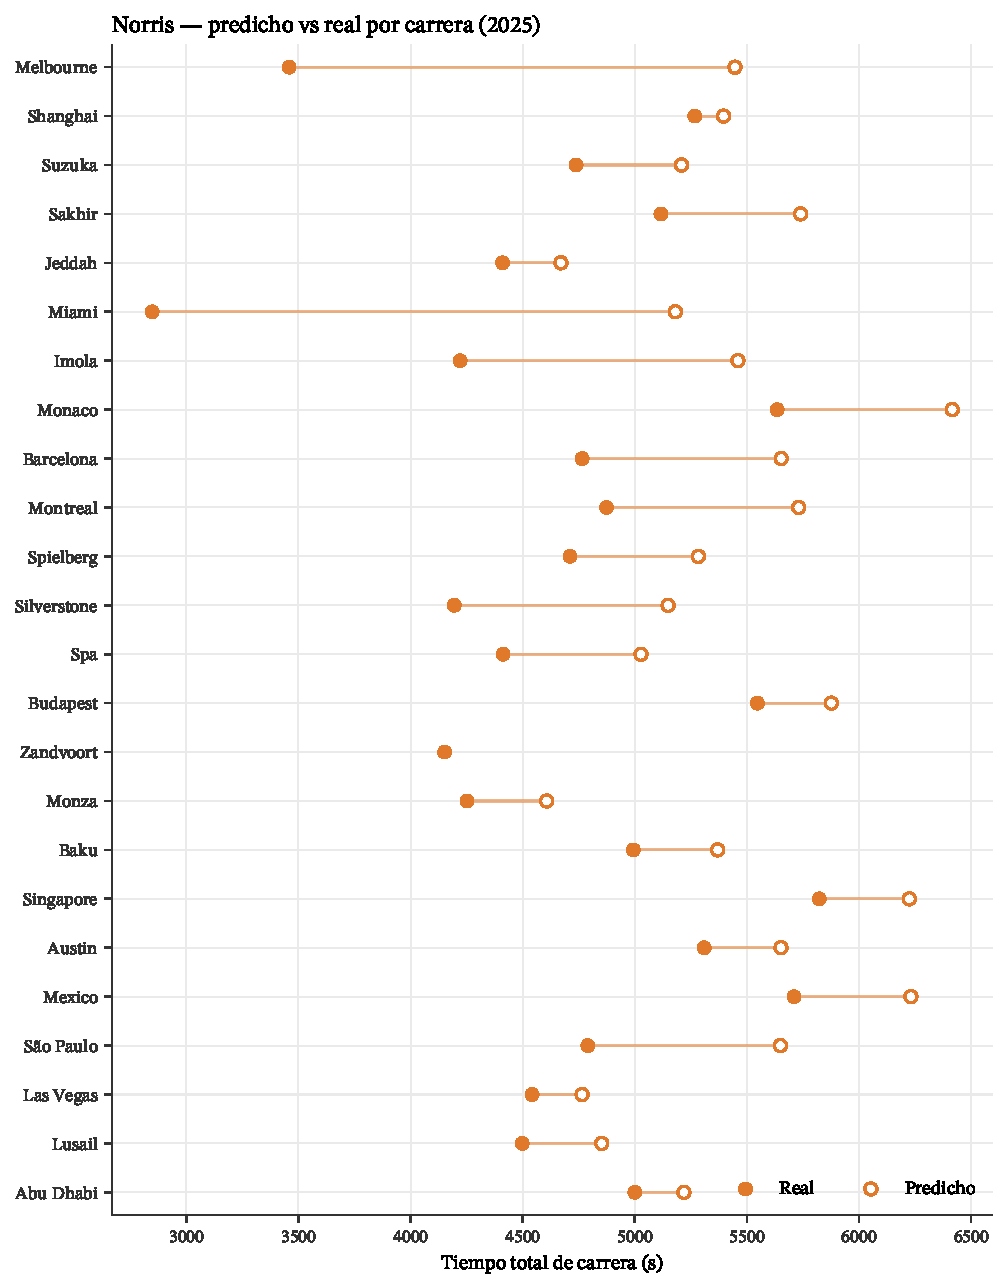
\includegraphics[height=0.85\textheight,keepaspectratio]{Chapter5/images/dumbbell_NOR.pdf}%
}{\rule{0pt}{5cm}}
\caption{Norris: tiempo predicho (círculo blanco) frente al tiempo real (círculo relleno) carrera a carrera, con el error firmado anotado a la derecha.}
\label{fig:eval_NOR_dumbbell}
\end{figure}

\clearpage
\begin{figure}[H]
\centering
\IfFileExists{Chapter5/images/dumbbell_PIA.pdf}{%
  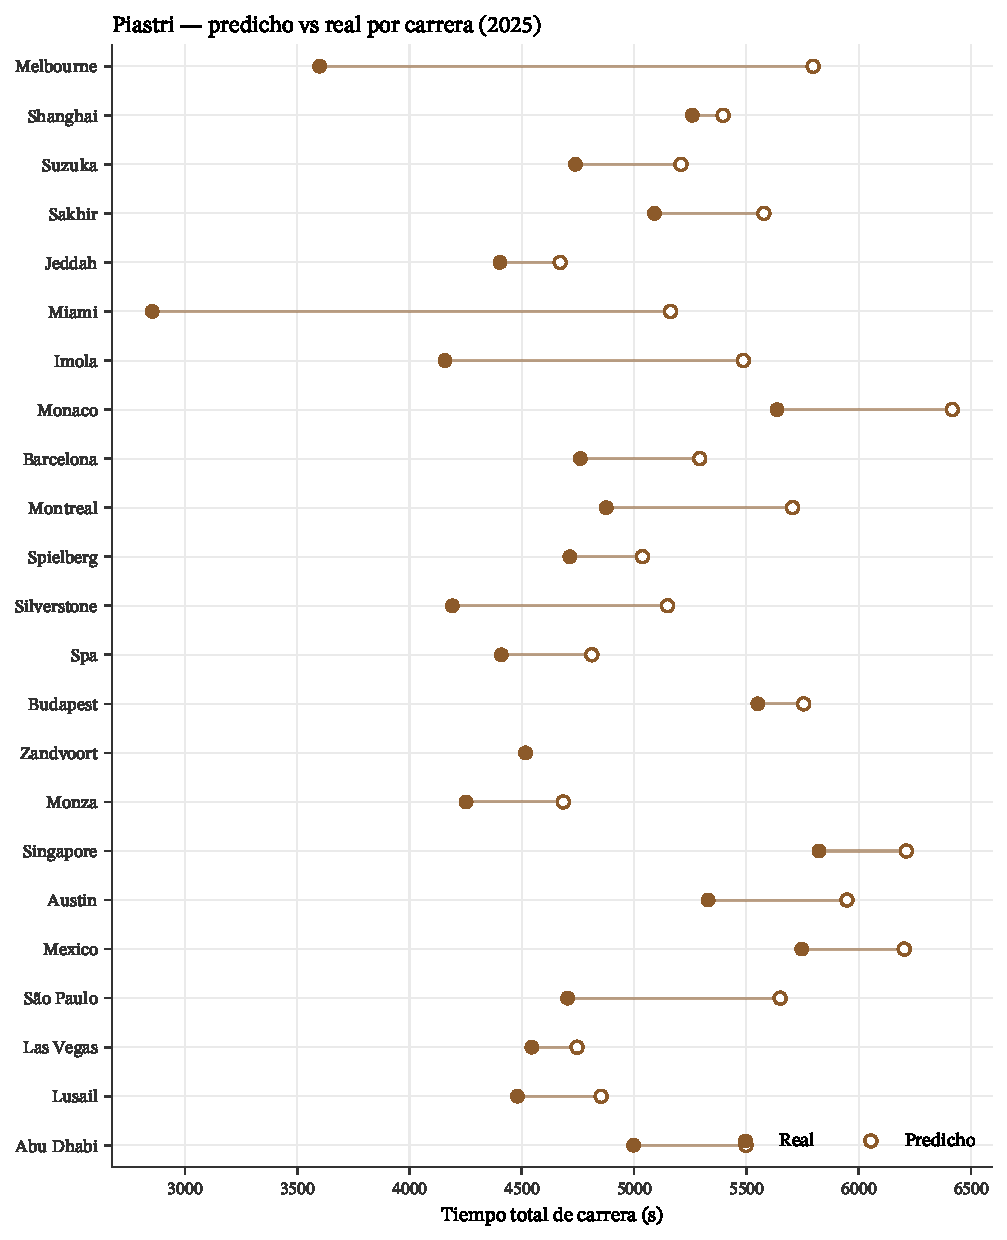
\includegraphics[height=0.85\textheight,keepaspectratio]{Chapter5/images/dumbbell_PIA.pdf}%
}{\rule{0pt}{5cm}}
\caption{Piastri: tiempo predicho frente al tiempo real carrera a carrera, con el error firmado anotado a la derecha.}
\label{fig:eval_PIA_dumbbell}
\end{figure}

\clearpage
\begin{figure}[H]
\centering
\IfFileExists{Chapter5/images/dumbbell_VER.pdf}{%
  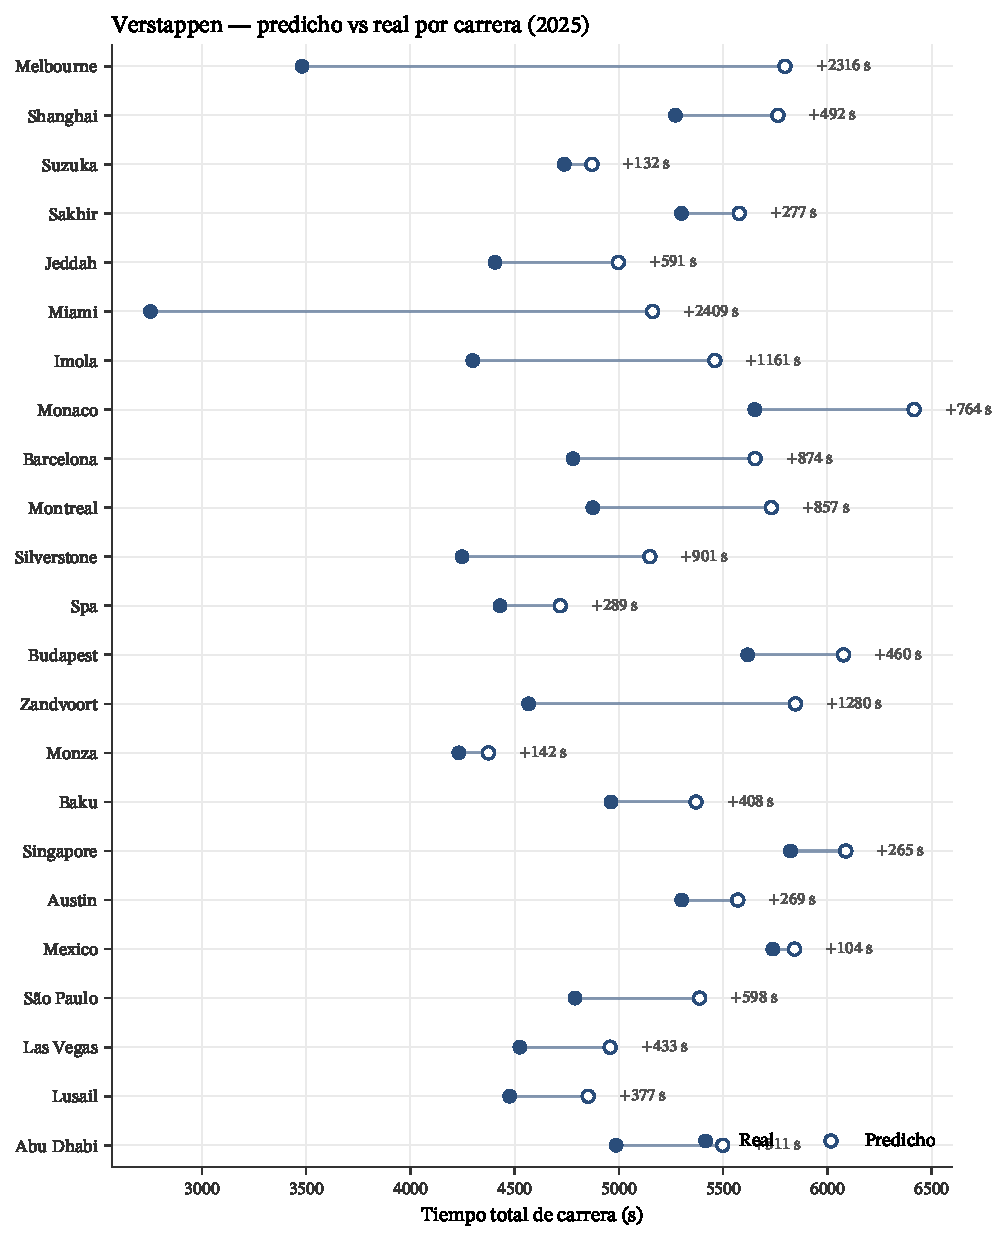
\includegraphics[height=0.85\textheight,keepaspectratio]{Chapter5/images/dumbbell_VER.pdf}%
}{\rule{0pt}{5cm}}
\caption{Verstappen: tiempo predicho frente al tiempo real carrera a carrera, con el error firmado anotado a la derecha.}
\label{fig:eval_VER_dumbbell}
\end{figure}

\clearpage
\begin{figure}[H]
\centering
\IfFileExists{Chapter5/images/dumbbell_LEC.pdf}{%
  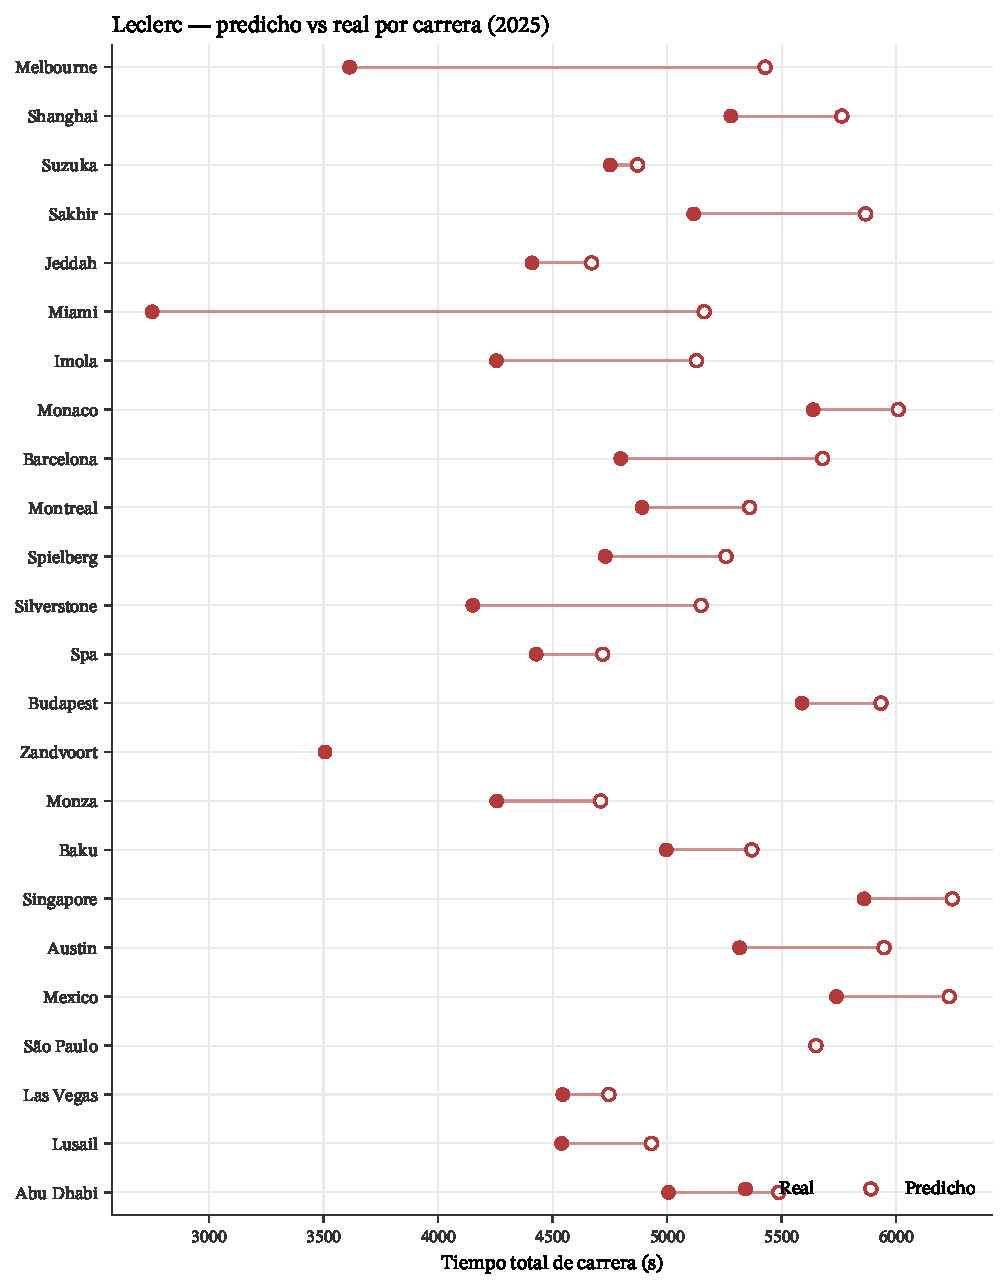
\includegraphics[height=0.85\textheight,keepaspectratio]{Chapter5/images/dumbbell_LEC.pdf}%
}{\rule{0pt}{5cm}}
\caption{Leclerc: tiempo predicho frente al tiempo real carrera a carrera, con el error firmado anotado a la derecha.}
\label{fig:eval_LEC_dumbbell}
\end{figure}
